\chapter{M\'etodos Computacionales y Experimentales} \label{cap:Metodos}
\section{M\'etodos computacionales} \label{Met:sec:mcomp}
Para poder implementar la teor\'ia descrita en el cap\'itulo \ref{cap:DFT} se utiliza el software libre Quantum-Espresso \cite{Giannozzi_2009,Giannozzi_2017}, el cual permite realizar c\'alculos de propiedades de materiales utilizando t\'ecnicas de primeros principios. Para poderlo emplear  es necesario realizar un modelo con la estructura at\'omica del material en cuesti\'on y  por este motivo es necesario crear una supercelda cuya elaboraci\'on se explica en la subsecci\'on \ref{Met:subsec:supercelda} y los detalles computacionales se explican en la secci\'on \ref{Met:subsec:detcomp}.
\subsection{Supercelda}  \label{Met:subsec:supercelda}
Para realizar una supercelda se  parte de la  celda unitaria del cristal que se puede obtener de bases de datos  de c\'alculos de primeros principios \cite{Jain2013}. Las superceldas son creadas utilizando el software VESTA \cite{Momma:db5098} y para visualizar dichas estructuras y las distribuciones de carga y magnetizaci\'on se utiliza XcrySDen \cite{kokalj_1999}.  En el presente trabajo se quieren estudiar las propiedades magn\'eticas inducidas por defectos y deformaciones en los siguientes materiales: Disulfuro de Vanadio $VS_2  \cite{osti_1308135} $, Diseleniuro de Vanadio$~VSe_2 \cite{osti_1284665}$, Disulfuro de Platino$~PtS_2 \cite{osti_1292393}$ y Diseleniuro de Platino $PtSe_2 \cite{osti_1187595}$, en primer lugar se crearon las superceldas  unitarias que son utilizadas para estudiar las propiedades magn\'eticas de los materiales sin vacancias. Para elaborarlas simplemente se desplaza la celda unitaria  para colocar el metal de transici\'on entre dos calcogenuros y posteriormente se la agrega una capa de vac\'io. En la figura \ref{Met:fig:SupU} se muestra esta estructura. 
\begin{figure}[hbt!]
	\centering
	\subfigure[]{
		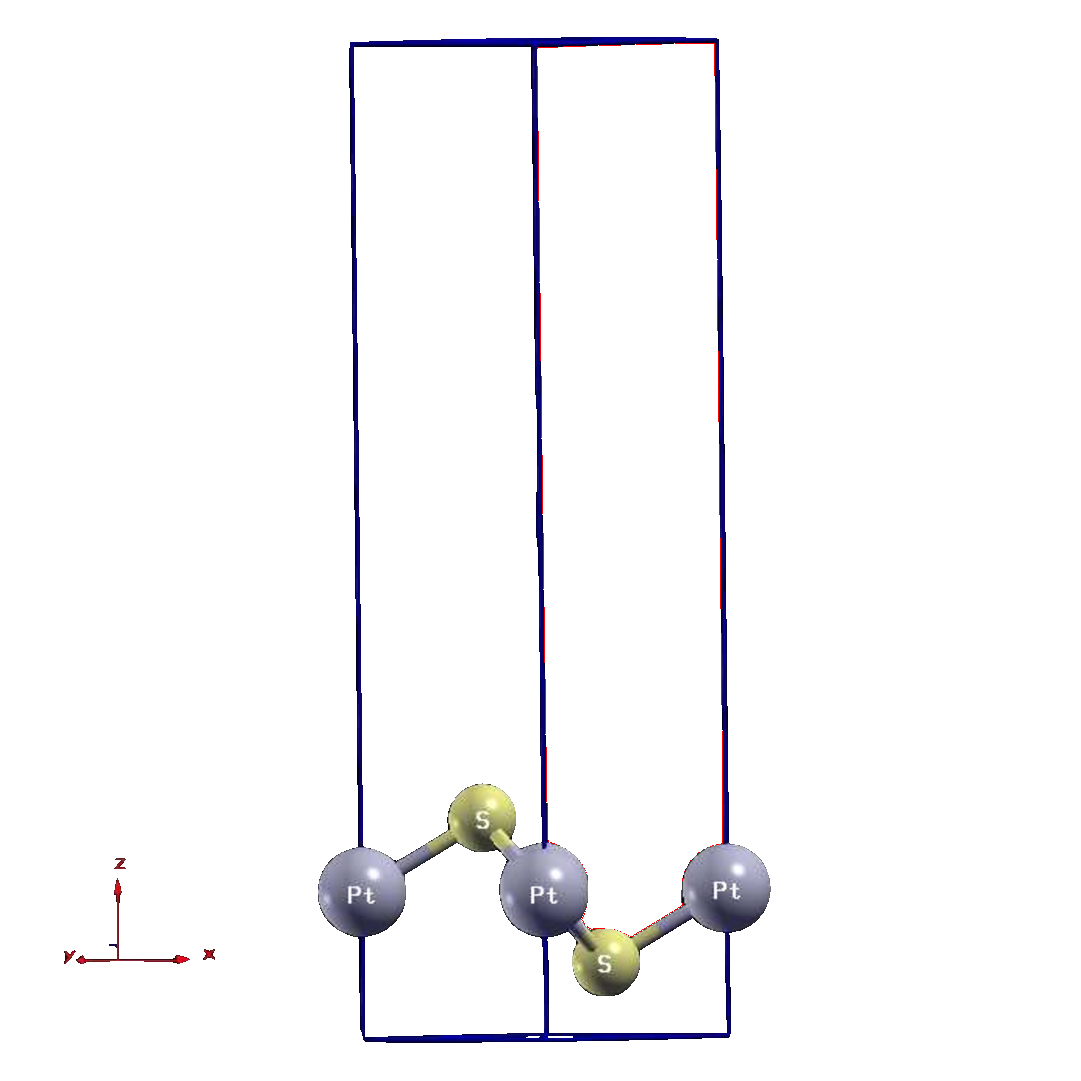
\epsfig{file=figMet/superceldaLado.eps, width=6.0cm,height=6.0cm}
		\label{Met:fig:supUcanto}
	}
    \subfigure[]{
    	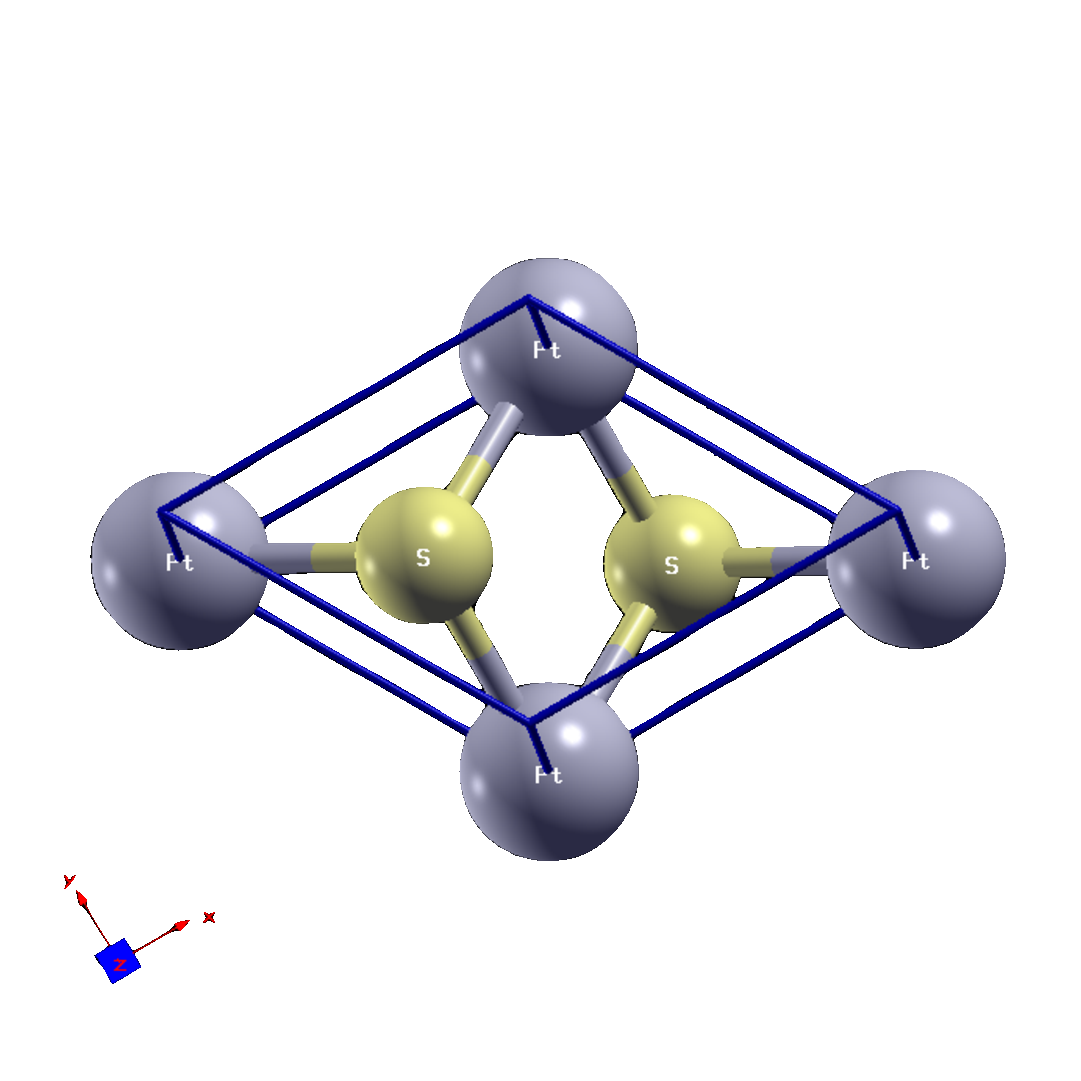
\epsfig{file=figMet/superceldaarriba.eps, width=6.0cm,height=6.0cm}
    	\label{Met:fig:supUarriba}
    }
    \caption[Supercelda de los materiales estudiados]{ Visualizaci\'on de la supercelda de $PtS_2$ vista de canto (\ref{Met:fig:supUcanto}) y desde arriba (\ref{Met:fig:supUarriba}). Por motivos visuales se agregan tres \'atomos de Platino.}
    \label{Met:fig:SupU}
\end{figure}   
\newline
\par  Para estudiar la vacancias del metal de transición, primeramente se crea una supercelda con cuatro celdas unitarias de tal forma que se tienen 12 \'atomos, cuatro metales de transici\'on y ocho calc\'ogenos y  se le agrega una capa de vac\'io. Posteriormente  se elimina un \'atomo del metal para crear la vacancia. En la figura \ref{Met:fig:SupV} se muestran los \'atomos en las posiciones en las que la energ\'ia y fuerza son m\'inimas en una supercelda con la vacancia de Platino; es decir est\'an optimizados (sec. \ref{sec:Fuerza}).
\begin{figure}[hbt!]
	\centering
	\subfigure[]{
		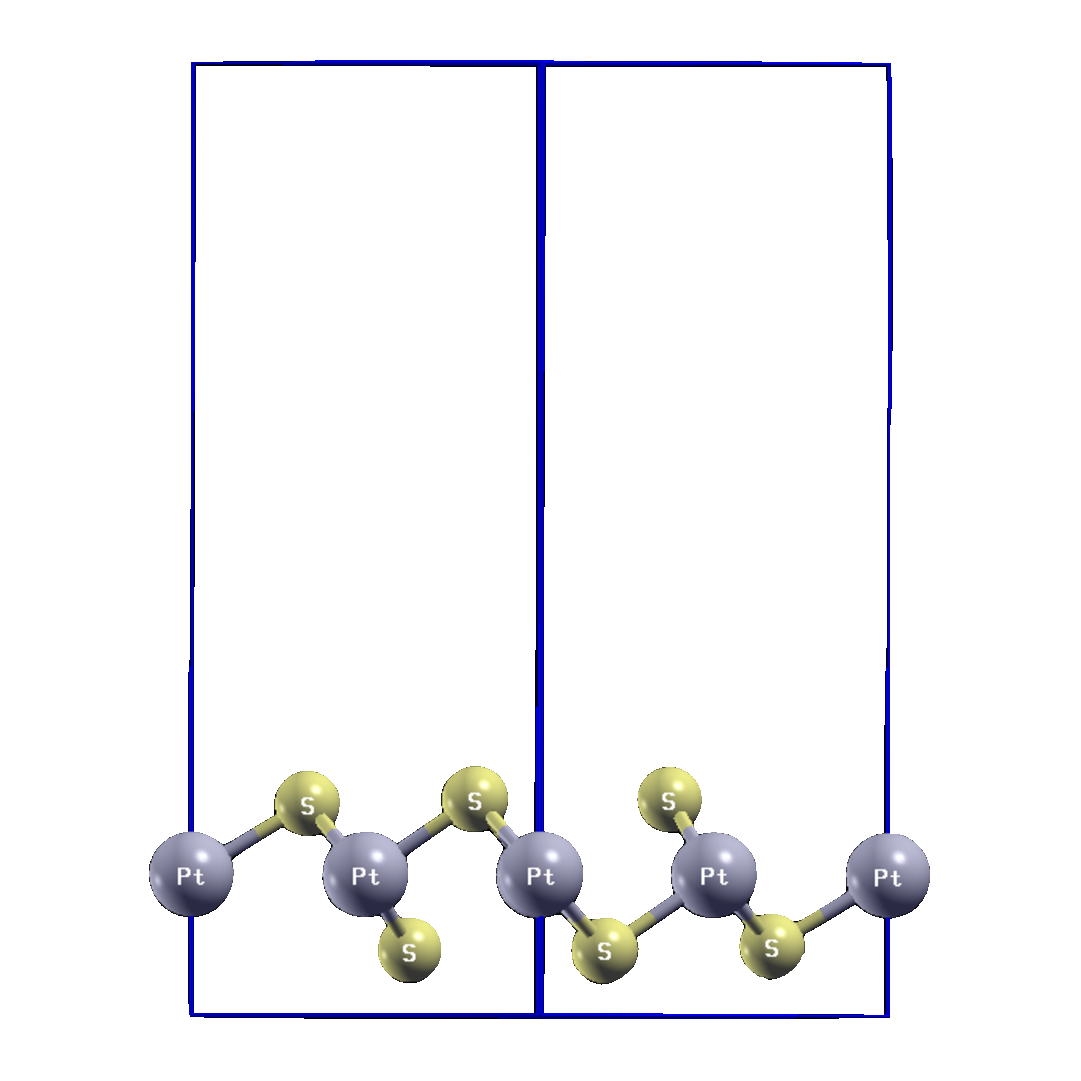
\epsfig{file=figMet/superceldaVacanciaLado.eps, width=7.0cm,height=7.0cm}
		\label{Met:fig:supVcanto}
	}
	\subfigure[]{
		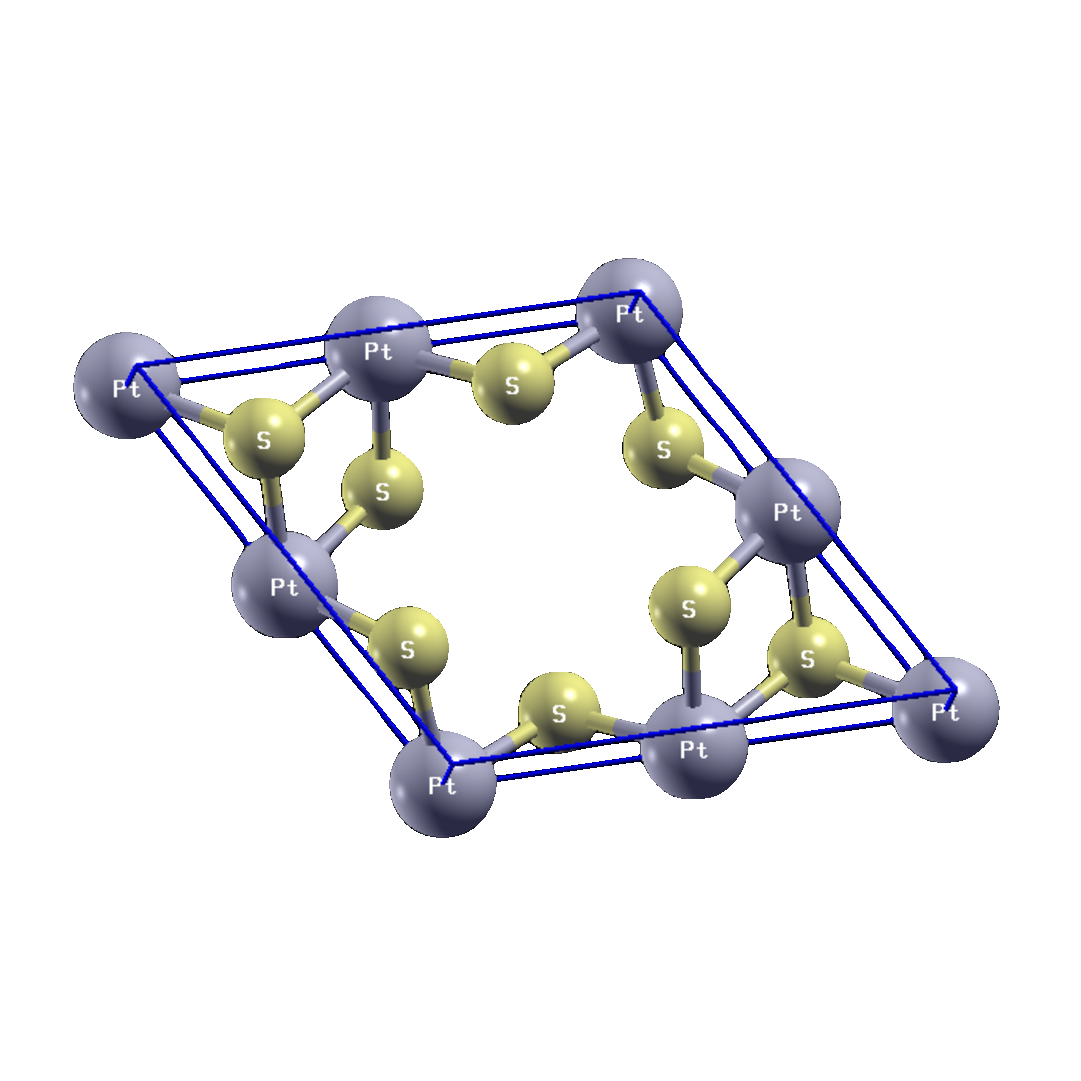
\epsfig{file=figMet/superceldaVacanciaArriba.eps, width=7.0cm,height=7.0cm}
		\label{Met:fig:supVarriba}
	}
	\caption[Estructura de la supercelda.]{ Visualizaci\'on de la supercelda de $PtS_2$  con vacancia de Pt en el software XcrySDen vista de canto (\ref{Met:fig:supVcanto}) y desde arriba (\ref{Met:fig:supVarriba}). Por motivos visuales se agregan tres \'atomos de Platino.}
	\label{Met:fig:SupV}
\end{figure}
\subsection{Detalles computacionales} \label{Met:subsec:detcomp}
  Se utiliz\'o el software de Quantum-Espresso en dos computadoras que se encuentran equipadas con un procesador con 8 n\'ucleos y 32 GB de memoria RAM. Esto permite realizar c\'alculos de forma paralelizada aunque el tama\~no de las celdas no pueden ser muy grandes. Debido a que es necesario optimizar geom\'etricamente las superceldas descritas anteriormente, se tiene que considerar el acople spin-\'orbita que afecta principalmente a los \'atomos de metales de transici\'on  y debido a esto, tambi\'en tiene una gran influencia en las posiciones en equilibrio de todos los \'atomos en la supercelda. Por lo tanto todos los c\'alculos que impliquen  alguna optimizaci\'on geom\'etrica se realizan considerando el acople spin-\'orbita.
  \newline
  \par De acuerdo a lo descrito en la secci\'on \ref{sec:pseudo} es necesario utilizar los pseudopotenciales para poder realizar los c\'alculos. En este caso se utilizan los pseudopotenciales PAW (Subsec. \ref{subsec:PAW}) y la aproximaci\'on PBE para el funcional de intercambio y correlaci\'on $E_{XC}$. Para el desarrollo de este trabajo se utilizaron los pseudopotenciales proporcionados por Quantum-Espresso  para c\'alculos escalares  y  completamente relativistas.
  \newline
  \par Antes de realizar cualquier c\'alculo es necesario el valor adecuado para la energ\'ia de corte y del n\'umero de puntos en la red de Monkhorst y Pack. La manera de realizar estas optimizaciones es realizando varios c\'alculos variando estos par\'ametros hasta que la energ\'ia total del sistema converja a un valor. En la tabla \ref{Met:Tab:Eckk1} se muestran los valores para la energ\'ia de corte  y el mapeo en el espacio rec\'iproco. Se puede observar que estos par\'ametros son mayores para los compuestos con Vanadio, lo cual se debe a que se trata de materiales con el orbital $3d$ en la banda de valencia, lo cual provoca que se necesiten mas ondas planas para poder describir las propiedades del material. As\'i mismo, se observa que n requieren utilizar mas puntos en el espacio reciproco,  una consecuencia a lo dicho anteriormente.  
  \begin{table} [!h]
  	\centering
  	\caption[Valores de la energ\'ia de corte y mapeo de Monkhorst-Pack.]{Muestra los valores para la energ\'ia de corte y el mapeo en el espacio rec\'iproco (mapeo de Monkhorst y Pack) para las estructuras utilizadas en este trabajo.}
  	\begin{tabular}{|c|c|m{5 cm}|} 
  		\hline
  		Material       &   $E_{corte}~~(Ry)$     & mapeo de Monkhorst y Pack $(k\times k \times 1)$  \\
  		\hline
  		\hline
  		$PtS_2$        &   $60 $             &  $~~~~~~~~11 \times 11 \times 1$ \\
  		$PtSe_2$        &   $63 $             &  $~~~~~~~~11 \times 11 \times 1$ \\
  		$VS_2$        &   $80 $             &  $~~~~~~~~21 \times 21 \times 1$ \\
  		$VSe_2$        &   $84 $             &  $~~~~~~~~21 \times 21 \times 1$ \\
  		 \hline
  	\end{tabular}
    
    \label{Met:Tab:Eckk1}
  \end{table}
  \newline
  \par Una vez que se han definido estas cantidades, es necesario realizar una optimizaci\'on geom\'etrica de la celda unitaria para encontrar las posiciones  de equilibrio de los \'atomos desde el punto de vista de Quantum-Espresso. Una vez que ya se ha logrado, esto se crea la supercelda con una vacancia (fig \ref{Met:fig:SupV}) y se realiza nuevamente una optimizaci\'on, pero en este caso se mantiene el volumen constante de tal forma que solo se desplazan los \'atomos a su nueva posici\'on de equilibrio.
  \newline
  \par Para estudiar el efecto de las  deformaciones en estos materiales, tanto con vacancia como sin ella, en la magnetizaci\'on se utiliza la siguiente ecuaci\'on
  \begin{equation}
  \varepsilon = \frac{a-a_0}{a_0}, \label{Met:ec:strain}
  \end{equation} 
  en donde $a$ es la magnitud del eje deformado y $a_0$ es sin deformar. Se utilizaron dos clases de deformaciones: una es la isotr\'opica en cual la deformaci\'on est\'a en la direcci\'on de los ejes cristalogr\'aficos $a$ y $b$, tal como se muestra en la figura \ref{Met:fig:strainiso}. Con el fin de  estudiar qu\'e sucede si se cambia el \'angulo de $120$° entre los ejes $a$ y $b$, adem\'as de tratar de simular una deformaci\'on mas real se aplica la deformaci\'on orientada a los ejes cartesianos $x$ y $y$ sujeta a la condici\'on $\varepsilon_y = -\varepsilon_x$, de tal forma que se puede utilizar la analog\'ia de cuando ``se aplasta un tubo con un fluido".  Dicha deformaci\'on se muestra en la figura \ref{Met:fig:strainanis}.
  \begin{figure}[hbt!]
  	\centering
     \subfigure[]{
     	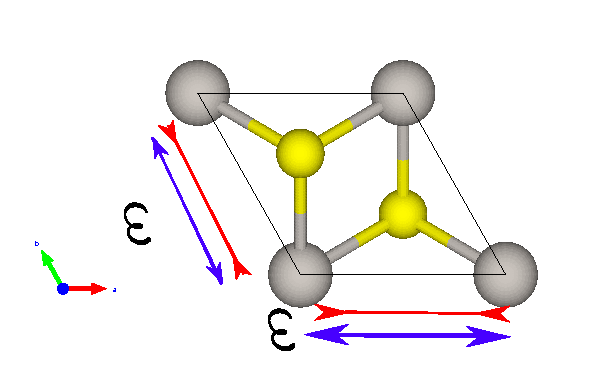
\epsfig{file=figMet/strainIso.eps, scale=0.9}
     	\label{Met:fig:strainiso}
     }
     \subfigure[]{
     	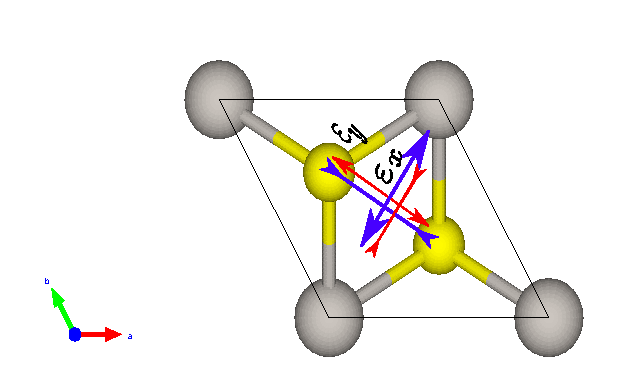
\epsfig{file=figMet/strainIAnis.eps, scale=0.9}
     	\label{Met:fig:strainanis}
     }	
     \caption[Deformaciones estudiadas.]{Deformaciones estudiadas en este trabajo. \ref{Met:fig:strainiso} Muestra la aplicaci\'on de una deformaci\'on isotr\'opica en direcci\'on de los ejes cristalinos y \ref{Met:fig:strainanis} una deformaci\'on dirigida en la direcci\'on de los ejes cartesianos.}
  \end{figure}
  \newline
  \par Como se dijo en las secci\'on \ref{subsec:nscf} es necesario utilizar la evaluaci\'on no auto-consistente para poder calcular la densidad de estados  y la estructura de bandas debido a que se requiere una cantidad mayor de puntos en el espacio rec\'iproco en comparaci\'on con el c\'alculo de la energ\'ia total del sistema. Para el caso de la densidad de estados  se utilizan $50 \times 50 \times 1 $ en la red de Monkhorst y Pack y  se utiliza un algoritmo de ajuste del tetraedro. Para el diagrama de bandas es necesario indicar el camino a seguir en la primera zona de Brillouin, en la figura \ref{Mat:fig:espacioK}. Se muestra \'esta indicando los puntos especiales y sus coordenadas en el espacio rec\'iproco. El camino que se sigui\'o para las estructuras de $PtS_2$ y $PtSe_2$ es $K-\Gamma-M-K$  y para las de $VS_2$ y $VSe_2$ es $\Gamma-M-K-\Gamma$. Es importante considerar que en el caso de que se aplique la deformaci\'on que se muestra en la figura \ref{Met:fig:strainanis}, el punto $M$ var\'ia linealmente de $(0.3518~0.3518~0)$ para $\varepsilon_x=-0.05$, a $(0.321~0.321~0)$ para $\varepsilon_x=0.04$. 
  \begin{figure}[hbt!]
  	\centering
  	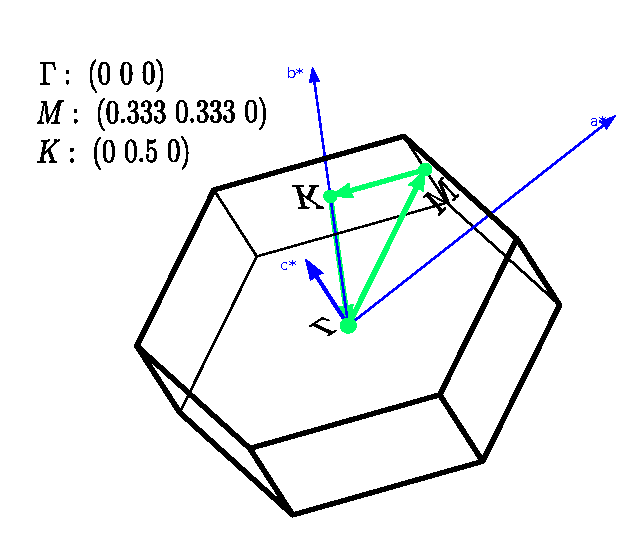
\epsfig{file=figMet/espacioK2.eps, width=8.0cm,height=8.0cm }
  	\caption[Puntos especiales en la zona de Brillouin.]{Mapeo en la primera zona de Brillouin indicando las coordenadas en el espacio rec\'iproco. Visualizado en XcrySDen}
    \label{Mat:fig:espacioK}
  \end{figure}
  \newline
  \par Para  generar las gr\'aficas de la estructura de bandas y de la densidad de estados, Quantum-Espresso cuenta con los  programas llamados bands.x y dos.x, los cuales toman los valores calculados por una evaluaci\'on no auto-consistente para poder generar las gr\'aficas correspondientes. Tambi\'en es importante obtener la densidad de estados proyectada en los orbitales at\'omicos (pDOS)  ya que de \'estos se puede observar cuales son los que contribuyen a la magnetizaci\'on. Para calcular el pDOS se utiliza el programa llamado projdos.x, el cual tambi\'en permite calcular la densidad de estados proyectada resuelta en el espacio rec\'iproco. De esta se puede obtener c\'omo es la contribuci\'on de cierto orbital a la estructura de bandas as\'i como cu\'ales bandas cuentan con spines orientados positiva y negativamente ($\uparrow,~\downarrow$).
  \newline
  \par Tambi\'en es de inter\'es visualizar la diferencia de densidad de electrones en el sistema para poder estudiar los enlaces qu\'imicos entre los \'atomos. Esta diferencia est\'a dada por la resta entre la densidad de electrones (ec. \ref{ec:densTot}) y la superposici\'on de las densidades at\'omicas.  As\'i mismo, tambi\'en es posible observar la densidad de la magnetizaci\'on resuelto en el espacio utilizando la ecuaci\'on \ref{ec:magn}, estas dos visualizaciones se pueden realizar utilizando una herramienta de Quantum Espresso llamada ``PostProc" (pp.x) y se puede observar en XcrySDen.
  
\section{M\'etodos experimentales} \label{Met:secmetExp}
\subsection{Montaje experimental}\label{Met:subsec:MontExp}
En la figura \ref{Met:fig:kerr} se muestra el montaje experimental utilizado para medir el efecto Kerr magneto-\'optico en configuraci\'on longitudinal. El sistema est\'a pensado para realizar mediciones variando el campo magn\'etico externo, las cuales son \'utiles para caracterizar las propiedades magn\'eticas del los materiales; es decir funcionar\'ia como un magnet\'ometro y se puede variar la longitud de onda lo cual es de gran utilidad para caracterizar los cambios en las propiedades electr\'onicas de los materiales bajo la influencia de un campo magn\'etico externo.
\begin{figure}[!hbt]
	\centering
	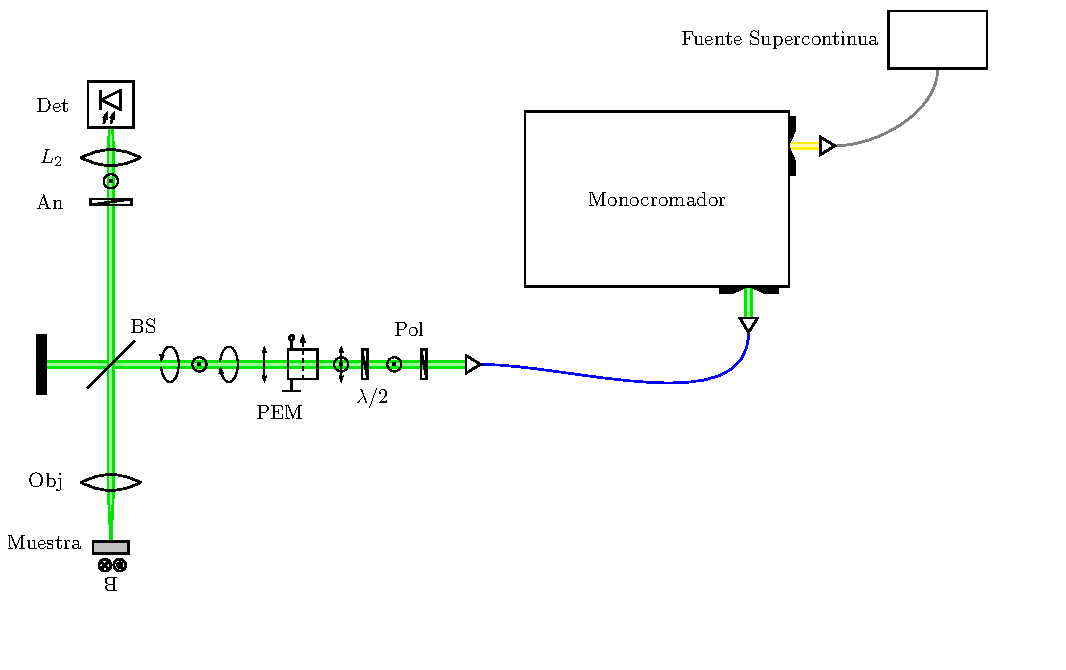
\includegraphics[scale=0.67]{figMet/diagrama/diagrama.pdf}
	\caption[Montaje experimental de espectroscop\'ia de efecto kerr magneto-\'optico.]{Montaje experimental para medir el efecto Kerr Mageto-\'optico en configuraci\'on longitudinal. La fiente supercontinua abarca un espectro de $430~nm $ a $2400~nm$ nm con una frecuencia de repetici\'on que var\'ia de $10~kHz $ a $80~MHz$ }
	\label{Met:fig:kerr}
\end{figure}
\newline
\par La fuente supercont\'inua es fabricada  por YSL Photonics y tiene como principales caracter\'isticas de que es posible controlar la frecuencia de repetici\'on y la potencia del pulso de salida, en el caso de este trabajo se utiliza una frecuencia de repetici\'on de $4 MHz$ al $30\%$  de la potencia total del pulso. El haz de esta fuente de luz sale colimado de una fibra \'optica y se introduce en un monocromador Acton 500M, el cual cuenta con tres rejillas de 300, 600 y 1200 $lineas/mm.$. En este caso se utilizan la de 1200 para el rango visible y la de 600 para el infrarrojo cercano. Este dispositivo se puede controlar por computadora mediante la comunicaci\'on serial. A la salida del monocromador se acopla el haz a una fibra \'optica para introducirlo en el sistema de medici\'on. A la salida de la fibra se utiliza una lente para colimar el haz y  posteriormente se coloca un polarizador Wollatson que est\'a orientado a $0\degree$ con respecto a la horizontal de tal forma que la polarizaci\'on del haz de salida est\'a polarizada linealmente. Debido a que es necesario orientar la direcci\'on de polarizaci\'on a $45 \degree$ se utiliza un retardador de media onda colocado en una montura rotatoria K10CR1/M de Thorlabs la cual puede ser controlada remotamente por medio del software Kinesis. Posteriormente se utiliza un modulador fotoel\'astico (PEM), cuyo eje r\'apido est\'a a $90 \degree$ con respecto al eje horizontal y cuyo  modelo es PEM-90 de Hinds Instruments, al cual se le puede controlar el retardo que se le induce al haz. En este caso se le agrega un retardo de $\lambda/4$ con una frecuencia de operaci\'on es de $42~ MHz$. Tambi\'en es posible controlarlo remotamente por medio de un puerto serial. Una vez que el haz sale del PEM se estar\'a modulando la polarizaci\'on del haz cambiando de una lineal a circular. Posteriormente se utiliza un beamsplitter para dirigir el haz hacia la muestra y se utiliza un objetivo de microscopio de 50x para enfocar la luz en la muestra que est\'a colocada entre un par de bobinas para inducir campo magn\'etico en la muestra en las direcciones marcadas en el figura \ref{Met:fig:kerr} y cuya magnitud se encuentra entre 0 y 0.7 mT. Dicho campo magn\'etico es controlado  variando la intensidad de corriente que circula a travez las bobinas y se cuenta con un controlador manual que tiene control PID para dicha corriente. El haz reflejado pasa por un segundo polarizador orientado a $90 \degree$ que funciona como analizador ya que convierte los cambios en polarizaci\'on en un cambio de intensidad y por \'ultimo, se utiliza una lente para enfocar la luz en un detector avalancha de Silicio de modelo  Thorlabs. La salida del detector se conecta a un mult\'imetro Keithley 720  y a un amplificador Lock in (sr510 Stanford Reseach) que se encuentra sincronizado con la frecuencia de operaci\'on del PEM. Ambos dispositivos pueden se pueden comunicar a una computadora por medio de un puerto GPIB-serial.
\newline 
\par Se utiliz\'o el an\'alisis de matrices de Jones (Ap\'endice \ref{Jones:App}) para deducir una expresi\'on de la intensidad de la luz que llega al detector y  se obtiene un par de expresiones para las razones de la intensidad que detecta el lock in cuando se encuentra sincronizado con el primer y segundo arm\'onico del retardo del modulador fotoel\'astico (ecs. \ref{Jones:ec:divI1} y\ref{Jones:ec:divI2} ):
\begin{eqnarray}
I_1/I_0 &=& 4 J_1 (\Psi_0) ~tan(\varPsi) ~(\theta_k ~sin(\Delta) - \eta_k~ cos(\Delta)) \label{Met:ec:divI1}\\
I_2/I_0 &=& -4 J_2 (\Psi_0) ~tan(\varPsi) ~(\theta_k~cos(\Delta) + \eta_k ~ sin(\Delta)) \label{Met:ec:divI2}.
\end{eqnarray}
En este caso $I_0$ es detectada por el mult\'imetro digital. Se utiliza un programa desarrollado en LabVIEW (Ap\'endice \ref{AppKerrAuto}), el cual es utilizado para controlar el monocromador  y el PEM as\'i como para adquirir informaci\'on del amplificador lock in y del mult\'imetro. Una vez que se tienen estos valores se realiza la raz\'on entre el valor del lock in y el del mult\'imetro de tal forma que se obtienen las expresiones \ref{Met:ec:divI1} y \ref{Met:ec:divI2} dependiendo de que si el lock in est\'a sincronizado a $f$ o $2f$.  Este programa le permite al usuario realizar mediciones variando la longitud de onda o medir el ciclo de hist\'eresis variando el campo magn\'etico externo aplicado a la muestra.
\subsection{An\'alisis de los datos experimentales} \label{Met:subsec:AnExp}
 De acuerdo con las ecuaciones \ref{Met:ec:divI1} y \ref{Met:ec:divI2} se observa que es necesario realizar un an\'alisis mas detallado debido a que no es posible obtener los valores  para la rotaci\'on ($\theta_k$) y la elipticidad ($\varepsilon_k$) Kerr de forma directa, dado  que en estas expresiones aparecen mezcladas en ambas ecuaciones. Es posible encontrar los valores para la rotaci\'on  y la elipticidad si se tratan las expresiones \ref{Met:ec:divI1} y \ref{Met:ec:divI2} como un sistema de ecuaciones, para lo cual es necesario conocer los valores de $\varPsi (eV)$ y $\Delta (eV)$ del beamsplitter. Estos valores fueron posible conocerlos realizando una medici\'on de elipsometr\'ia a $70\degree$ cuyos valores se observan en la figura \ref{Met:fig:ElipBS} junto con su ajuste realizado con el programa WVASE. En base con este ajuste es posible estimar los valores de $\varPsi (eV)$ y $\Delta (eV)$ para $45 \degree$ con ayuda de WVASE que se muestran en la figura \ref{Met:fig:ElipBS45}. Como se puede observar estos dos par\'ametros presentan grandes variaciones en todo el espectro  por lo que fue necesario implementar una rutina en Python (Ap\'endice \ref{App:Py}) para poder obtener  los valores de la elipticidad  y el \'angulo Kerr resolviendo el sistema de ecuaciones (\ref{Met:ec:divI1} y \ref{Met:ec:divI2}).
\begin{figure}[!hbt]
	\centering
	\subfigure[valores de $\Psi$]{
	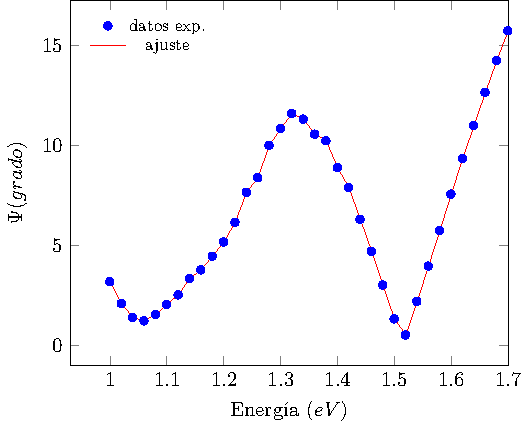
\includegraphics[scale=0.75]{figMet/figElips/grafPsi}
	\label{Met:fig:PsiBS}
	}
    \subfigure[valores de $\Delta$]{
    	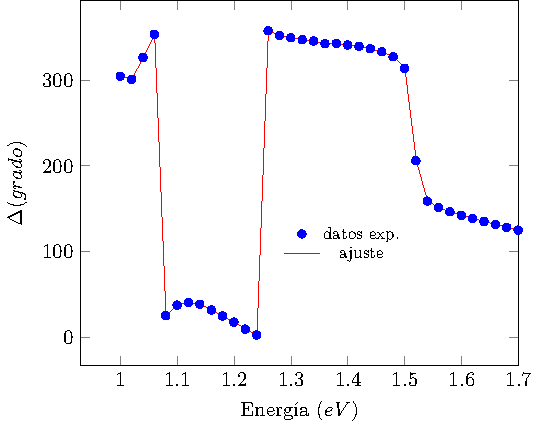
\includegraphics[scale=0.75]{figMet/figElips/grafTheta}
    	\label{Met:fig:DeltaBS}
    }
\caption[Gr\'aficas de $\Psi$ y $\Delta$ del beamspliter a $70 \degree$.]{valores experimentales a $70\degree$  para $\Psi$ y $\Delta$ del beamsplitter en funci\'on de la energ\'ia del fot\'on con su ajuste.} 
\label{Met:fig:ElipBS}
\end{figure}
\begin{figure}[!hbt]
	\centering
	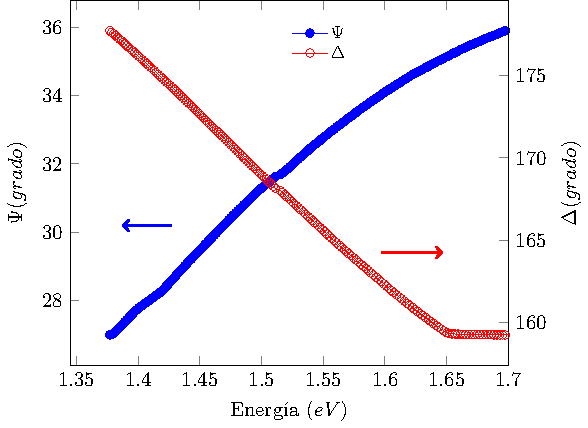
\includegraphics[scale=1.3]{figMet/figElips/grafPsidelta45.pdf}
	\caption[Gr\'aficas de $\Psi$ y $\Delta$ del beamspliter a $70 \degree$.]{valores calculados a $45\degree$  para $\Psi$ y $\Delta$ del beamsplitter.}
	\label{Met:fig:ElipBS45}
\end{figure}
\newline
\subsection{Muestras}\label{Met:subsec:Muest}
La muestra utilizada en para comprobar que el funcionamiento del sistema de espectroscop\'ia de efecto Kerr Magneto-\'optico es una aleaci\'on de Hierro, Cobalto y Boro (CoFeB)	en donde las concentraciones son del $20~\%$ para el Cobalto y el Boro y del $60~\%$ para el Hierro. Dado que se aplica un campo magn\'etico externo B es necesario conocer la respuesta en funci\'on del campo magn\'etico $H$, es conocido que se relacionan con la siguiente expresi\'on \cite{magMan_1}
\begin{equation}
	\pmb{B}_{[T]}=\mu_0 (\pmb{H}_{[A ~m^{-1}]}+\pmb{M}_{[A ~m^{-1}]} + \pmb{H}_d ),
	\label{Met:ec:BSI}
\end{equation}  
	en donde $\pmb{B}$ es el campo magn\'etico externo, $\pmb{H}$ es el campo  magn\'etico inducido, $\pmb{M}$ es la magnetizaci\'on y $\pmb{H}_d$ es el campo desmagnetizante definido como $\pmb{H}_d = -N_d \pmb{M}$ en donde   $N_d$ es el factor desmagnetizante que generalmente depende de la geometr\'ia de la estructura, la ecuaci\'on \ref{Met:ec:BSI} puede ser escrita en unidades CGS \cite{magMan_1}
    \begin{equation}
    	\pmb{B}_{[Gauss]}= \pmb{H}_{[Oe]}+4 \pi \pmb{M}_{[emu ~cm^{-3}]} +\pmb{H}_d ,
    	\label{Met:ec:BCGS}
    \end{equation}	
en donde hay que considerar que las unidades SI se relacionan con las CGS de la siguiente manera \cite{magMan_2}:
\begin{eqnarray}
	1~T&=& 10^{-4}~ Gauss \nonumber \\
	1~ A~m^{-1} &=& 4 \pi \times 10^{-3}~ Oe \nonumber \\
	1~emu~cm^{-3} &=& 10^{-3} A~ m^{-1}. \nonumber
\end{eqnarray}
Dado que se trata de una pel\'icula delgada de CoFeB en este caso el factor desmagnetizante en el caso que el campo  magnético  externo $\pmb{B}$ se dirija en la direcci\'on $x$ se obtiene \cite{magMan_1}, $N_{d,y}=N_{d,x}=0$ y $N_{d,z}=4\pi$ en unidades CGS, entonces la ecuaci\'on \ref{Met:ec:BCGS} se puede aproximar a
\begin{equation*}
	\pmb{B} \approx \pmb{H}.
\end{equation*} 
  \endinput
